% questions.tex —— 2010 年·全国新课标卷·理科 · 题目内容片段（无答案）
% 由 tools/generate_projects.py 依来源总账自 2010/2010_数学真题_全国新课标理_试题.md 生成，勿手改（改源 MD 后重跑）


\gkpart{数学}

\begin{gktip}
\textbf{来源说明}：本题面依据固定源 PDF 两页 A3 题面逐题转录，原卷印刷页码 615–616。固定源不附答案，答案和解析均由本库独立复算。

\textbf{图形说明}：第 4、7、18、22、24 题的原卷图形或流程图重绘为 TikZ/PGFPlots 矢量图。图形标记所指的 PNG 不随仓库保存。
\end{gktip}

\gkpart{一、选择题}

\begin{question}
\gkti{1}已知集合 $A=\{x\mid |x|\leq2, x\in\mathbb R\}$，$B=\{x\mid \sqrt{x}\leq4, x\in\mathbb Z\}$，则 $A\cap B=$\mbox{（　　）}

（A）$(0,2)$\quad（B）$[0,2]$\quad（C）$\{0,2\}$\quad（D）$\{0,1,2\}$

\end{question}
\begin{question}
\gkti{2}已知复数 $z=\left(\dfrac{\sqrt3+i}{1-\sqrt3i}\right)^2$，$\bar z$ 是 $z$ 的共轭复数，则 $z\cdot\bar z=$\mbox{（　　）}

（A）$\dfrac14$\quad（B）$\dfrac12$\quad（C）$1$\quad（D）$2$

\end{question}
\begin{question}
\gkti{3}曲线 $y=\dfrac{x}{x+2}$ 在点 $(-1,-1)$ 处的切线方程为\mbox{（　　）}

（A）$y=2x+1$\quad（B）$y=2x-1$\quad（C）$y=-2x-3$\quad（D）$y=-2x-2$

\Needspace{0.4\textheight}
\end{question}
\begin{question}
\gkti{4}如图，质点 $P$ 在半径为 $2$ 的圆周上逆时针运动，其初始位置为 $P_0(\sqrt2,-\sqrt2)$，角速度为 $1$，那么点 $P$ 到 $x$ 轴的距离 $d$ 关于时间 $t$ 的函数图象大致为\mbox{（　　）}
\nopagebreak[4]
\begin{center}% 2010 全国卷理科第 4 题：质点圆周运动的四个函数图象选项。
\begin{tikzpicture}[font=\scriptsize, line width=0.35pt]
  \begin{scope}[shift={(0,0)}]
    \draw[->] (0,0) -- (3.8,0) node[right] {$t$};
    \draw[->] (0,0) -- (0,2.35) node[above] {$d$};
    \draw[domain=0:3.35, samples=100, smooth, variable=\tau]
      plot (\tau,{2*abs(sin(deg(\tau)))});
    \node[below left] at (0,0) {O}; \node at (0.2,2.55) {A};
  \end{scope}
  \begin{scope}[shift={(4.9,0)}]
    \draw[->] (0,0) -- (3.8,0) node[right] {$t$};
    \draw[->] (0,0) -- (0,2.35) node[above] {$d$};
    \draw[domain=0:3.35, samples=100, smooth, variable=\tau]
      plot (\tau,{2*abs(sin(deg(\tau+45)))});
    \node[below left] at (0,0) {O}; \node at (0.2,2.55) {B};
  \end{scope}
  \begin{scope}[shift={(0,-3.0)}]
    \draw[->] (0,0) -- (3.8,0) node[right] {$t$};
    \draw[->] (0,0) -- (0,2.35) node[above] {$d$};
    \draw[domain=0:3.35, samples=100, smooth, variable=\tau]
      plot (\tau,{2*abs(sin(deg(\tau-45)))});
    \node[below left] at (0,0) {O}; \node at (0.2,2.55) {C};
  \end{scope}
  \begin{scope}[shift={(4.9,-3.0)}]
    \draw[->] (0,0) -- (3.8,0) node[right] {$t$};
    \draw[->] (0,0) -- (0,2.35) node[above] {$d$};
    \draw[domain=0:3.35, samples=100, smooth, variable=\tau]
      plot (\tau,{2*abs(cos(deg(\tau)))});
    \node[below left] at (0,0) {O}; \node at (0.2,2.55) {D};
  \end{scope}
\end{tikzpicture}
\end{center}
\nopagebreak[4]
（A）图 A\quad（B）图 B\quad（C）图 C\quad（D）图 D

\end{question}
\begin{question}
\gkti{5}已知命题 $p_1$：函数 $y=2^x-2^{-x}$ 在 $\mathbb R$ 为增函数；$p_2$：函数 $y=2^x+2^{-x}$ 在 $\mathbb R$ 为减函数。则在命题 $q_1=p_1\lor p_2$，$q_2=p_1\land p_2$，$q_3=(\lnot p_1)\lor p_2$ 和 $q_4=p_1\land(\lnot p_2)$ 中，真命题是\mbox{（　　）}

（A）$q_1,q_3$\quad（B）$q_2,q_3$\quad（C）$q_1,q_4$\quad（D）$q_2,q_4$

\end{question}
\begin{question}
\gkti{6}某种种子每粒发芽的概率都为 $0.9$，现播种了 $1000$ 粒，对于没有发芽的种子，每粒需再补种 $2$ 粒，补种的种子数记为 $X$，则 $X$ 的数学期望为\mbox{（　　）}

（A）$100$\quad（B）$200$\quad（C）$300$\quad（D）$400$

\Needspace{0.4\textheight}
\end{question}
\begin{question}
\gkti{7}如果执行如图所示的框图，输入 $N=5$，则输出的数等于\mbox{（　　）}
\nopagebreak[4]
\begin{center}% 2010 全国卷理科第 7 题：程序框图。
\begin{tikzpicture}[font=\footnotesize, >=Stealth, node distance=2.2mm, line width=0.4pt,
  box/.style={draw, minimum height=1.5em, minimum width=5.8em, inner xsep=6pt},
  term/.style={draw, rounded corners=6pt, minimum height=1.5em, inner xsep=8pt},
  io/.style={draw, trapezium, trapezium left angle=70, trapezium right angle=110,
             minimum height=1.5em, inner xsep=3pt},
  dec/.style={draw, diamond, aspect=2.6, inner sep=1.5pt}]
  \node[term] (start) {开始};
  \node[io, below=of start] (input) {输入 $N$};
  \node[box, below=of input] (init) {$k=1,\ S=0$};
  \node[box, below=of init] (step) {$S=S+\dfrac{1}{k(k+1)}$};
  \node[dec, below=of step] (cond) {$k<N$};
  \node[box, right=16mm of cond] (inc) {$k=k+1$};
  \node[io, below=9mm of cond] (output) {输出 $S$};
  \node[term, below=of output] (end) {结束};
  \draw[->] (start) -- (input);
  \draw[->] (input) -- (init);
  \draw[->] (init) -- (step);
  \draw[->] (step) -- (cond);
  \draw[->] (cond.east) -- node[above] {是} (inc.west);
  \draw[->] (inc.north) |- (step.east);
  \draw[->] (cond.south) -- node[right] {否} (output.north);
  \draw[->] (output) -- (end);
\end{tikzpicture}
\end{center}
\nopagebreak[4]
（A）$\dfrac54$\quad（B）$\dfrac45$\quad（C）$\dfrac65$\quad（D）$\dfrac56$

\end{question}
\begin{question}
\gkti{8}设偶函数 $f(x)$ 满足 $f(x)=x^3-8$（$x\geq0$），则 $\{x\mid f(x-2)>0\}=$\mbox{（　　）}

（A）$\{x\mid x<-2\text{ \text{或} }x>4\}$\quad（B）$\{x\mid x<0\text{ \text{或} }x>4\}$

（C）$\{x\mid x<0\text{ \text{或} }x>6\}$\quad（D）$\{x\mid x<-2\text{ \text{或} }x>2\}$

\end{question}
\begin{question}
\gkti{9}若 $\cos\alpha=-\dfrac45$，$\alpha$ 是第三象限的角，则
$\dfrac{1+\tan\dfrac\alpha2}{1-\tan\dfrac\alpha2}=$\mbox{（　　）}

（A）$-\dfrac12$\quad（B）$\dfrac12$\quad（C）$2$\quad（D）$-2$

\end{question}
\begin{question}
\gkti{10}设三棱柱的侧棱垂直于底面，所有棱长都为 $a$，顶点都在一个球面上，则该球的表面积为\mbox{（　　）}

（A）$\pi a^2$\quad（B）$\dfrac73\pi a^2$\quad（C）$\dfrac{11}3\pi a^2$\quad（D）$5\pi a^2$

\end{question}
\begin{question}
\gkti{11}已知函数

\nopagebreak[4]
\[
f(x)=\begin{cases}
|\lg x|,&0<x\leq10,\\
-\dfrac12x+6,&x>10,
\end{cases}
\]

若 $a\text{、}b\text{、}c$ 互不相等，且 $f(a)=f(b)=f(c)$，则 $abc$ 的取值范围是\mbox{（　　）}

（A）$(1,10)$\quad（B）$(5,6)$\quad（C）$(10,12)$\quad（D）$(20,24)$

\end{question}
\begin{question}
\gkti{12}已知双曲线 $E$ 的中心为原点，$F(3,0)$ 是 $E$ 的焦点，过 $F$ 的直线 $l$ 与 $E$ 相交于 $A\text{、}B$ 两点，且 $AB$ 的中点为 $N(-12,-15)$，则 $E$ 的方程为\mbox{（　　）}

（A）$\dfrac{x^2}{3}-\dfrac{y^2}{6}=1$\quad（B）$\dfrac{x^2}{4}-\dfrac{y^2}{5}=1$\quad（C）$\dfrac{x^2}{6}-\dfrac{y^2}{3}=1$\quad（D）$\dfrac{x^2}{5}-\dfrac{y^2}{4}=1$

\end{question}
\gkpart{二、填空题}

\begin{question}
\gkti{13}设 $y=f(x)$ 为区间 $[0,1]$ 上的连续函数，且恒有 $0\leq f(x)\leq1$，可以用随机模拟方法近似计算积分 $\displaystyle\int_0^1f(x)\,dx$。先产生两组（每组 $N$ 个）区间 $[0,1]$ 上的均匀随机数 $x_1,x_2,\ldots,x_N$ 和 $y_1,y_2,\ldots,y_N$，由此得到 $N$ 个点 $(x_i,y_i)$（$i=1,2,\ldots,N$），再数出其中满足 $y_i\leq f(x_i)$ 的点数 $N_1$，那么由随机模拟方法可得积分 $\displaystyle\int_0^1f(x)\,dx$ 的近似值为\gkblank{}。

\end{question}
\begin{question}
\gkti{14}正视图为一个三角形的几何体可以是\gkblank{}。（写出三种）

\end{question}
\begin{question}
\gkti{15}过点 $A(4,1)$ 的圆 $C$ 与直线 $x-y-1=0$ 相切于点 $B(2,1)$，则圆 $C$ 的方程为\gkblank{}。

\end{question}
\begin{question}
\gkti{16}在 $\triangle ABC$ 中，$D$ 为边 $BC$ 上一点，$BD=\dfrac12DC$，$\angle ADB=120^\circ$，$AD=2$。若 $\triangle ADC$ 的面积为 $3-\sqrt3$，则 $\angle BAC=$\gkblank{}。

\end{question}
\gkpart{三、解答题}

\begin{question}
\gkti{17}设数列 $\{a_n\}$ 满足 $a_1=2$，$a_{n+1}-a_n=3\cdot2^{2n-1}$。

（1） 求数列 $\{a_n\}$ 的通项公式；

（2） 令 $b_n=na_n$，求数列 $\{b_n\}$ 的前 $n$ 项和 $S_n$。

\Needspace{0.4\textheight}
\end{question}
\begin{question}
\gkti{18}如图，已知四棱锥 $P-ABCD$ 的底面为等腰梯形，$AB\parallel CD$，$AC\perp BD$，垂足为 $H$，$PH$ 是四棱锥的高，$E$ 为 $AD$ 中点。
\nopagebreak[4]
\begin{center}% 2010 全国卷理科第 18 题：等腰梯形底面的四棱锥示意图。
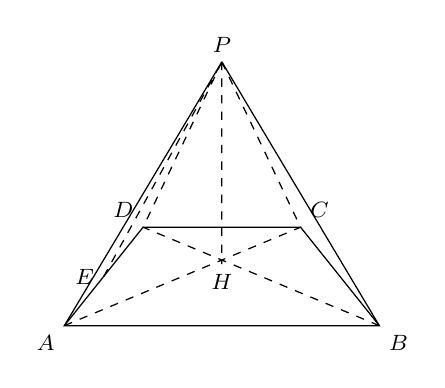
\begin{tikzpicture}[font=\footnotesize, line width=0.45pt]
  \coordinate (A) at (0,0);
  \coordinate (B) at (4.0,0);
  \coordinate (D) at (1.0,1.25);
  \coordinate (C) at (3.0,1.25);
  \coordinate (H) at (2.0,0.78);
  \coordinate (P) at (2.0,3.35);
  \coordinate (E) at (0.5,0.625);
  \draw (A)--(B)--(C)--(D)--cycle;
  \draw[dashed] (A)--(C) (B)--(D) (P)--(H) (P)--(D) (P)--(C) (E)--(P);
  \draw (P)--(A) (P)--(B);
  \node[below left] at (A) {$A$};
  \node[below right] at (B) {$B$};
  \node[above left] at (D) {$D$};
  \node[above right] at (C) {$C$};
  \node[above] at (P) {$P$};
  \node[below] at (H) {$H$};
  \node[left] at (E) {$E$};
\end{tikzpicture}
\end{center}
\nopagebreak[4]
（1） 证明：$PE\perp BC$；

（2） 若 $\angle APB=\angle ADB=60^\circ$，求直线 $PA$ 与平面 $PEH$ 所成角的正弦值。

\end{question}
\begin{question}
\gkti{19}为调查某地区老人是否需要志愿者提供帮助，用简单随机抽样方法从该地区调查了 $500$ 位老年人，结果如下：

\begin{center}
\begin{tabular}{lrr}
\toprule
性别 & 男 & 女 \\
\midrule
需要 & 40 & 30 \\
不需要 & 160 & 270 \\
\bottomrule
\end{tabular}
\end{center}

（1） 估计该地区老年人中，需要志愿者提供帮助的老年人的比例；

（2） 能否有 $99\%$ 的把握认为该地区的老年人是否需要志愿者提供帮助与性别有关？

（3） 根据（2）的结论，能否提供更好的调查方法来估计该地区老年人需要志愿者帮助的比例？说明理由。

\Needspace{10\baselineskip}
附：

\begin{center}
\begin{tabular}{lrrr}
\toprule
$P(K^2\geq k)$ & $0.050$ & $0.010$ & $0.001$ \\
\midrule
$k$ & $3.841$ & $6.635$ & $10.828$ \\
\bottomrule
\end{tabular}
\end{center}

\nopagebreak[4]
\[
K^2=\frac{n(ad-bc)^2}{(a+b)(c+d)(a+c)(b+d)}.
\]

\end{question}
\begin{question}
\gkti{20}设 $F_1\text{、}F_2$ 分别是椭圆 $E:\dfrac{x^2}{a^2}+\dfrac{y^2}{b^2}=1$（$a>b>0$）的左、右焦点，过 $F_1$ 且斜率为 $1$ 的直线 $l$ 与 $E$ 相交于 $A\text{、}B$ 两点，且 $|AF_2|\text{、}|AB|\text{、}|BF_2|$ 成等差数列。

（1） 求 $E$ 的离心率；

（2） 设点 $P(0,-1)$ 满足 $|PA|=|PB|$，求 $E$ 的方程。

\end{question}
\begin{question}
\gkti{21}设函数 $f(x)=e^x-1-x-ax^2$。

（1） 若 $a=0$，求 $f(x)$ 的单调区间；

（2） 若当 $x\geq0$ 时 $f(x)\geq0$，求 $a$ 的取值范围。

\Needspace{0.4\textheight}
\end{question}
\begin{question}
\gkti{22}如图，已知圆上的弧 $\widehat{AC}=\widehat{BD}$，过 $C$ 点的圆的切线与 $BA$ 的延长线交于 $E$ 点，证明：
\nopagebreak[4]
\begin{center}% 2010 全国卷理科第 22 题：圆、切线与 BA 的延长线示意图。
\begin{tikzpicture}[font=\footnotesize, line width=0.45pt]
  \coordinate (O) at (2.25,1.85);
  \def\r{1.65}
  \coordinate (A) at (0.95,0.83);
  \coordinate (B) at (0.62,2.75);
  \coordinate (C) at (3.35,3.05);
  \coordinate (D) at (3.78,1.02);
  \coordinate (E) at (5.05,0.45);
  \draw (O) circle (\r);
  \draw (A)--(B)--(C)--(D)--cycle;
  \draw (B)--(A)--(E);
  \draw (C)--(E);
  \draw[dashed] (O)--(C);
  \node[below left] at (A) {$A$};
  \node[left] at (B) {$B$};
  \node[above right] at (C) {$C$};
  \node[below right] at (D) {$D$};
  \node[right] at (E) {$E$};
  \node[below] at (O) {$O$};
  \draw ($(C)!0.12!(E)$) -- ++(-0.17,-0.29);
\end{tikzpicture}
\end{center}
\nopagebreak[4]
（1） $\angle ACE=\angle BCD$；

（2） $BC^2=BE\cdot CD$。

\end{question}
\begin{question}
\gkti{23}已知直线 $C_1$：

\nopagebreak[4]
\[
x=1+t\cos\alpha,\qquad y=t\sin\alpha\quad(t\text{ \text{为参数}}),
\]

\Needspace{5\baselineskip}
圆 $C_2$：

\nopagebreak[4]
\[
x=\cos\theta,\qquad y=\sin\theta\quad(\theta\text{ \text{为参数}}).
\]

（1） 当 $\alpha=\dfrac\pi3$ 时，求 $C_1$ 与 $C_2$ 的交点坐标；

（2） 过坐标原点 $O$ 作 $C_1$ 的垂线，垂足为 $A$，$P$ 为 $OA$ 的中点，当 $\alpha$ 变化时，求点 $P$ 轨迹的参数方程，并指出它是什么曲线。

\Needspace{0.4\textheight}
\end{question}
\begin{question}
\gkti{24}设函数 $f(x)=|2x-4|+1$。

（1） 画出函数 $y=f(x)$ 的图象；

（2） 若不等式 $f(x)\leq ax$ 的解集非空，求 $a$ 的取值范围。
\nopagebreak[4]
\begin{center}% 2010 全国卷理科第 24 题：y=|2x-4|+1。
\begin{tikzpicture}[font=\footnotesize, line width=0.45pt]
  \draw[->] (-0.5,0) -- (4.6,0) node[right] {$x$};
  \draw[->] (0,0) -- (0,5.4) node[above] {$y$};
  \draw[thick] (0,5) -- (2,1) -- (4.2,5.4);
  \fill (2,1) circle (1.2pt);
  \node[below] at (2,0) {$2$};
  \node[left] at (0,1) {$1$};
  \node[below left] at (0,0) {$O$};
\end{tikzpicture}
\end{center}
\nopagebreak[4]

\end{question}